\chapter{Algorithm Modifications}\label{chap:modif}
\section{Predicted-Variation of ABM} \label{sec:predABM}
As seen in section \ref{sec:ABM}, the ABM method needs to use a predicted value for every iteration; therefore, only if the solution converges, the value of $y$ that you obtained could be used as another predicted value for the variable and use it to obtain a more precise solution. So, the algorithm could keep doing this till the difference of the last predicted values reaches a small $\epsilon$ picked by the user or as it reaches a maximum iteration, so it is certain that the algorithm always terminates.

This modification does increase the accuracy (to which extent, it is gonna be discussed in this section) but it increases the run time of the method. 

\subsection{Chaotic Financial System}
In order to test this modification, the Financial System studied in example \ref{ex:finance} will be tested. The respective generalization to fractional-order differential equations, following \cite{chen2008nonlinear}, will be
\begin{equation}
    \begin{cases}
    \mathcal{D}_c^{\alpha_1} x=z+(y-a)x&\\
    \mathcal{D}_c^{\alpha_2} y=1-by-x^2&\\
    \mathcal{D}_c^{\alpha_3} z=-x-cz&
    \end{cases}
\end{equation}

The simulations were performed using $(\alpha_1,\,\alpha_2,\,\alpha_3)=(1,\,1,\, 0.8)$, $(x_0,\,y_0,\,z_0)=(2,\,3,\,2)$, $T=200$ and $N=10000$. The parameters were chosen as $(a,\,b,\,c)=(3,\,0.1,\,1)$, in order to compare the results with \cite{chen2008nonlinear}. The simulations are shown in the following figures (\ref{fig:predictedFinancial} for time-series and \ref{fig:predictedFinancialXY} for $XY$ phase portrait):

\begin{figure}[H]
\centering
\begin{subfigure}[ht]{0.3\textwidth}
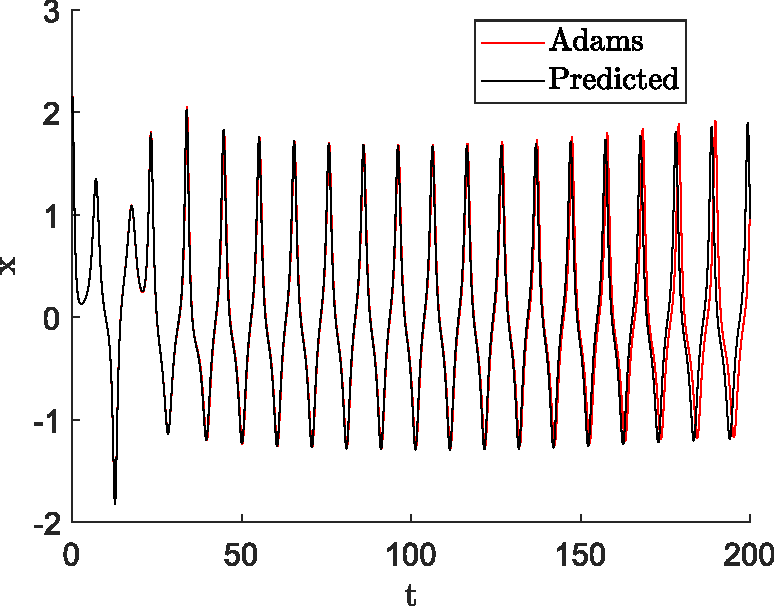
\includegraphics[scale=0.29]{files/adams_predicted_tx.pdf}
\end{subfigure}
\begin{subfigure}[ht]{0.3\textwidth}
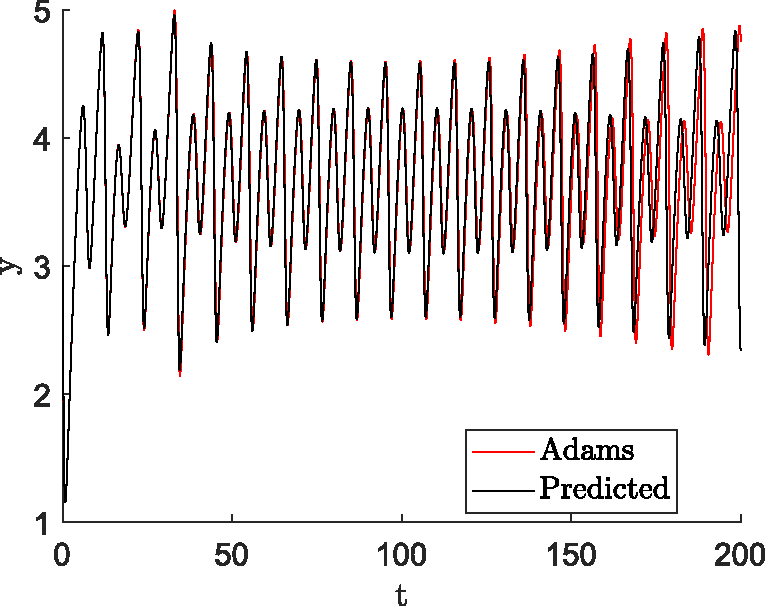
\includegraphics[scale=0.29]{files/adams_predicted_ty.pdf}
\end{subfigure}
\begin{subfigure}[ht]{0.3\textwidth}
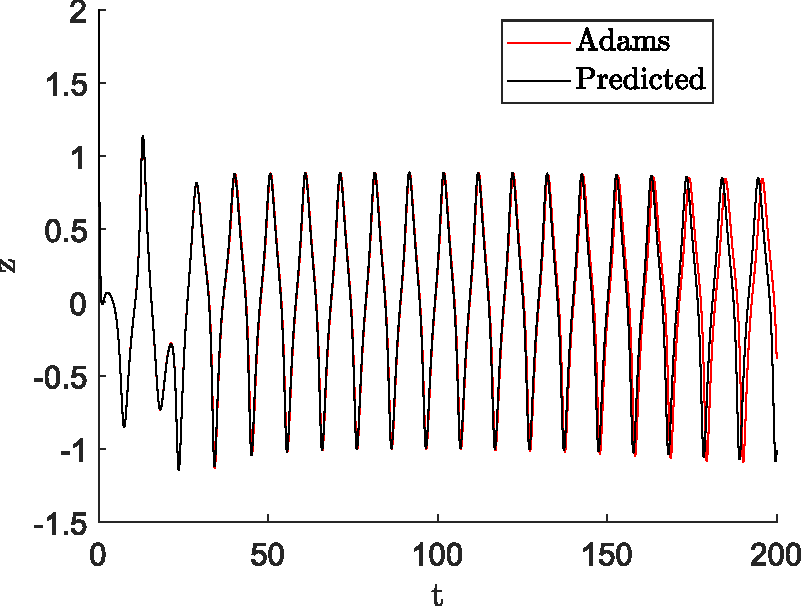
\includegraphics[scale=0.29]{files/adams_predicted_tz.pdf}
\end{subfigure}
\caption{Predicted modification compared with the original algorithm.}
\label{fig:predictedFinancial}
\end{figure}

\begin{figure}[H]
    \centering
    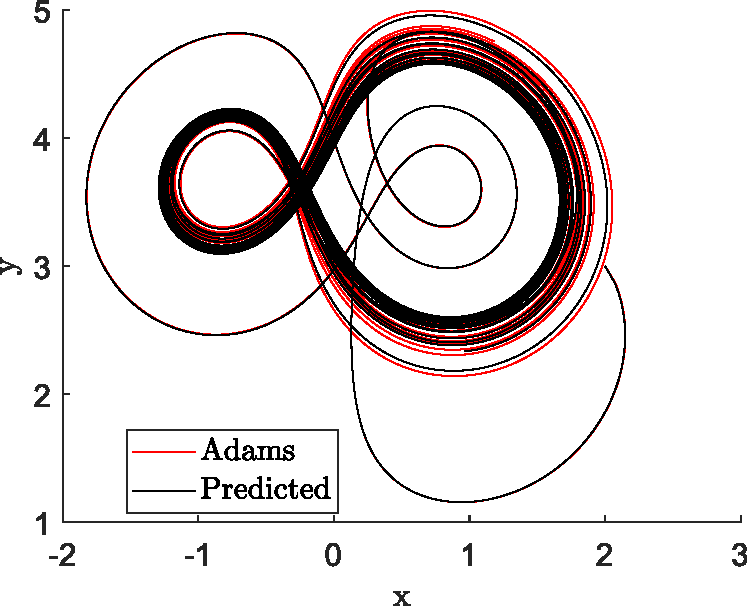
\includegraphics[scale=0.5]{files/adams_predicted_xy.pdf}
    \caption{Phase plane for the variables x and y.}
    \label{fig:predictedFinancialXY}
\end{figure}
This results show that this modification does not show significant improvement in this particular example. In figure \ref{fig:predictedFinancial}, the time series are shown for all state variables $x$, $y$ and $z$; note that both approximations overlap (generally). 

\subsection{Bagley-Torvik Equation}
The Bagley-Torvik equation is a model the describes the motion of a rigid plate in a Newtonian fluid, this equation was originally proposed in \cite{torvik1984appearance}. This model is given by
\begin{equation}
    Ay''(t)+B\mathcal{D}_c^{3/2}y(t)+Cy(t)=f(t)
\end{equation}

As Diethelm and Ford states in \cite{diethelm2002numerical}, if $f(t)=1+t$, the exact solution to this problem is given by
\begin{equation}
    y(t)=1+t
\end{equation}
For any choice of parameters $A$, $B$ and $C$.

Now we will use this result as a reference to compare the ABM method and the modification presented in this section. Following the ideas presented in section PHASE FRACTIONAL

The simulation was conducted based on \cite{diethelm2002numerical}, therefore, we chose $A=B=C=1$. The simulation was conducted, for the standard ABM method, with $T=10$, $N=15$; and, for the predicted scheme, with $T=10$, $N=15$, $\text{\texttt{tol}}=10^{-7}$ and $\text{\texttt{nmax}}=10$. The results are presented in figure \ref{fig:comparBagleyTorvik}.


\begin{figure}[H]
    \centering
    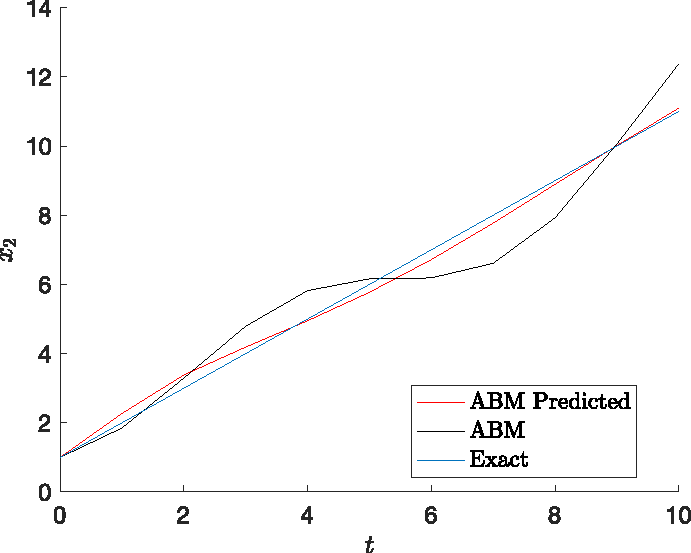
\includegraphics[scale=0.5]{files/comparPredictedABM.pdf}
    \caption{Comparison between the original and predicted scheme.}
    \label{fig:comparBagleyTorvik}
\end{figure}
